\chapter{Methodology}\label{chap:concl}
In this chapter, we present the methodology employed in the development of a simple banking application using Canisters on the Internet Computer. The aim of this project was to leverage the unique features and capabilities of Canisters to build a decentralized system for handling banking transactions and providing financial services to users.

\section{Platform Selection}
The decision to use the Internet Computer platform was driven by its decentralized nature, scalability, and robust security features. By utilizing the Technology Canister, which provides a secure and reliable environment for executing smart contracts and managing data, we were able to harness the power of the Internet Computer to build banking application. 

\begin{enumerate}
    \item \subsubsection{Internet Computer (IC)}
    The Internet Computer (IC) is a decentralized blockchain network that offers extensive computational power for executing canisters. This is made possible by a network of independent node providers who operate nodes across various data centers located around the world, ensuring scalability and distribution of resources.

    \item \subsubsection{Canister}  A canister is a unified entity that combines \ac{Wasm} \cite{webassemblywiki} program code and data storage. It is open for deployment by anyone on the Internet Computer. Canisters are stored and their code is executed in a replicated and fault-tolerant manner across multiple machines, known as nodes, within a subnet. In contrast to traditional blockchains, the Internet Computer allows for different mutability policies for smart contracts. A smart contract on the Internet Computer can adhere to various mutability policies, such as complete immutability (where no changes can be made by anyone), unilateral mutability (allowing changes to be made solely by the dApp developer), or \ac{DAO} mutability (permitting changes authorized by a decentralized autonomous organization).

    \item \subsubsection{Canister Cycles}
    Canisters pay, using cycles, for the \ac{IC} resources they consume. To this end, canisters need to be “topped up” with cycles. Cycles can be acquired with the ICP token, the \ac{IC}'s utility token. Buying cycles with ICP removes the ICP token from the supply and creates an amount of cycles with the corresponding value. One Trillion cycles can be acquired with ICP worth 1 XDR, where an XDR is a basket comprising major currencies and one XDR is roughly 1.3 USD as of Q3 2022.

    \item \subsubsection{Controller}The controller of a canister refers to an individual, organization, or another canister that holds administrative privileges over that specific canister. Controllers are distinguished by their principals. For instance, a canister's controller possesses the authority to upgrade the canister's WebAssembly \cite{webassemblywiki} code or delete the canister altogether.
    \item \subsubsection{Principal}
A principal is an entity that can be authenticated by the Internet Computer. This is the same sense of the word principal as the Wikipedia \cite{principalwiki} definition. Principals that interact with the Internet Computer do so using a certain identity.

    \item \subsubsection{Replica}
The replica is a collection of protocol components that are necessary for a node to participate in a subnet.
\end{enumerate}

\section{System Design}

The development process of the web banking applications on the Internet Computer began by conducting a detailed analysis of the requirements and specifications. We then proceeded to design a comprehensive system architecture due to Figure \ref{fig:DBanking application architecture.} that encompassed all the essential components for a secure and efficient web banking experience. This included user registration, robust data storage mechanisms, and robust authentication protocols.


\begin{figure}[H]
    \centering
    
    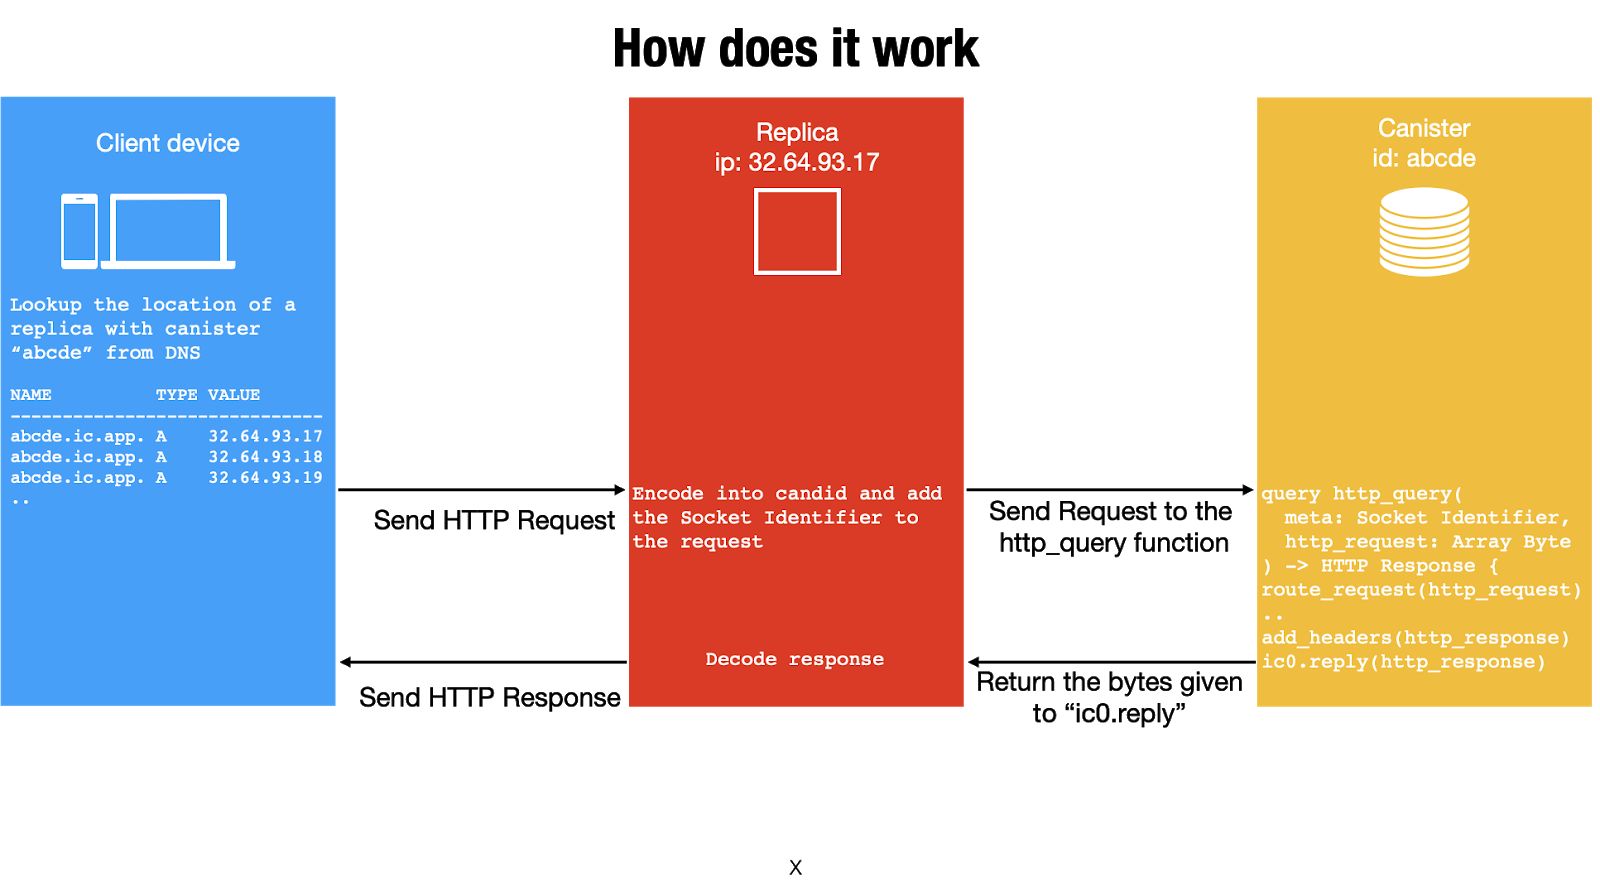
\includegraphics[width=0.8\textwidth]{IC-request.png}
    \caption{DBanking application architecture.}
    \label{fig:DBanking application architecture.}
\end{figure}


To ensure seamless integration and leverage the capabilities of the Internet Computer, the system was specifically designed to be compatible with the Technology Canister. By utilizing the features and functionalities provided by the Technology Canister, we were able to achieve a smooth and effective integration of the web banking applications into the Internet Computer ecosystem.

To gain a deeper understanding of the inner workings of \ac{HTTP} requests on the \ac{IC}, let's explore the underlying process. Initially, when a client device initiates a request to a website, the website's domain name is resolved via \ac{DNS}, resulting in a list of \ac{IP} addresses belonging to replica nodes that store the target canister. The complete \ac{HTTP} request is then forwarded to the appropriate replica, which proceeds to perform a query call to the canister. Subsequently, the canister responds with the \ac{HTTP} response, which is relayed back to the replica. Finally, the replica transmits the response to the end user's device, where it is decoded and presented as the relevant website information.

\section{Implementation}
We implemented the DBank application by developing the frontend using Node.js and the backend with Motoko programming language. With the power of Canister technology, we deployed the application onto the Internet Computer, providing users with a decentralized banking experience. Through this implementation, we aimed to create a user-friendly interface and robust functionality, enabling individuals worldwide to access and utilize the benefits of DBank. Join us as we delve into the details of implementing DBank and discover the potential of decentralized finance.
\subsubsection{Backend}
I implemented this application using the Motoko programming language. Motoko is specifically designed for developing smart contracts and is well-suited for the programming model of the Internet Computer. It offers seamless integration with the unique features of the blockchain, allowing developers to leverage its capabilities effectively.

Motoko is a strongly typed language that follows the actor-based model, enabling easy communication and collaboration among actors. It also includes built-in support for orthogonal persistence and asynchronous message passing. The language provides several productivity and safety features, such as automatic memory management, generics, type inference, pattern matching, and support for both arbitrary- and fixed-precision arithmetic.

Additionally, Motoko transparently utilizes the Internet Computer's Candid interface definition language and wire format. This enables typed, high-level, and cross-language interoperability, making it easier to communicate with other components or systems within the Internet Computer ecosystem.

By utilizing Motoko as shown in Figure \ref{fig:Implementation Code}, I was able to take advantage of its powerful features and the seamless integration it offers with the Internet Computer, ensuring both productivity and safety in developing the application.

\begin{figure}[H]
    \centering
    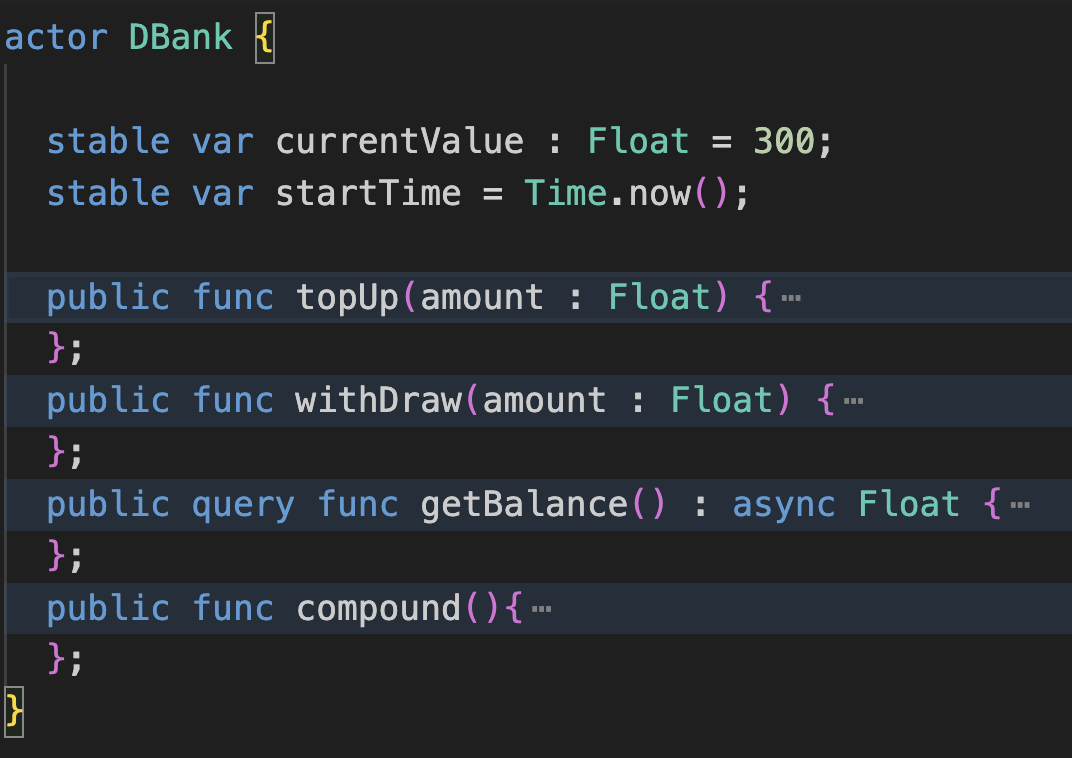
\includegraphics[width=0.8\textwidth]{Implementation.png}
    \caption{Implementation Code.}
    \label{fig:Implementation Code}
\end{figure}

In simple terms, the actor model is a conceptual framework for concurrent computing. It is a mathematical model that describes how individual actors behave when they receive messages. When an actor receives a message, it can perform certain actions such as updating its internal state, sending messages to other actors, or even creating new actors. Essentially, the actor model allows actors to communicate and collaborate by exchanging messages and modifying their own state based on the messages they receive.


The code snippet represents an implementation of an actor called DBank in the context of a banking application. Let's break down the code and explain it in a humanized manner:

The DBank actor is designed to manage a user's bank account. It has a couple of stable variables: \textit{currentValue} represents the current balance in the bank account, initialized to 300, and \textit{startTime} stores the time when the account was created.

The actor provides several functions to interact with the bank account.


The \textit{topUp} function as shown in Figure \ref{fig:Update Call} allows the user to deposit money into their account. The amount parameter specifies the amount of money to be deposited. The function increases the \textit{currentValue} by the deposited amount and prints the updated balance using the Debug.print function.

\begin{figure}[H]
    \centering
    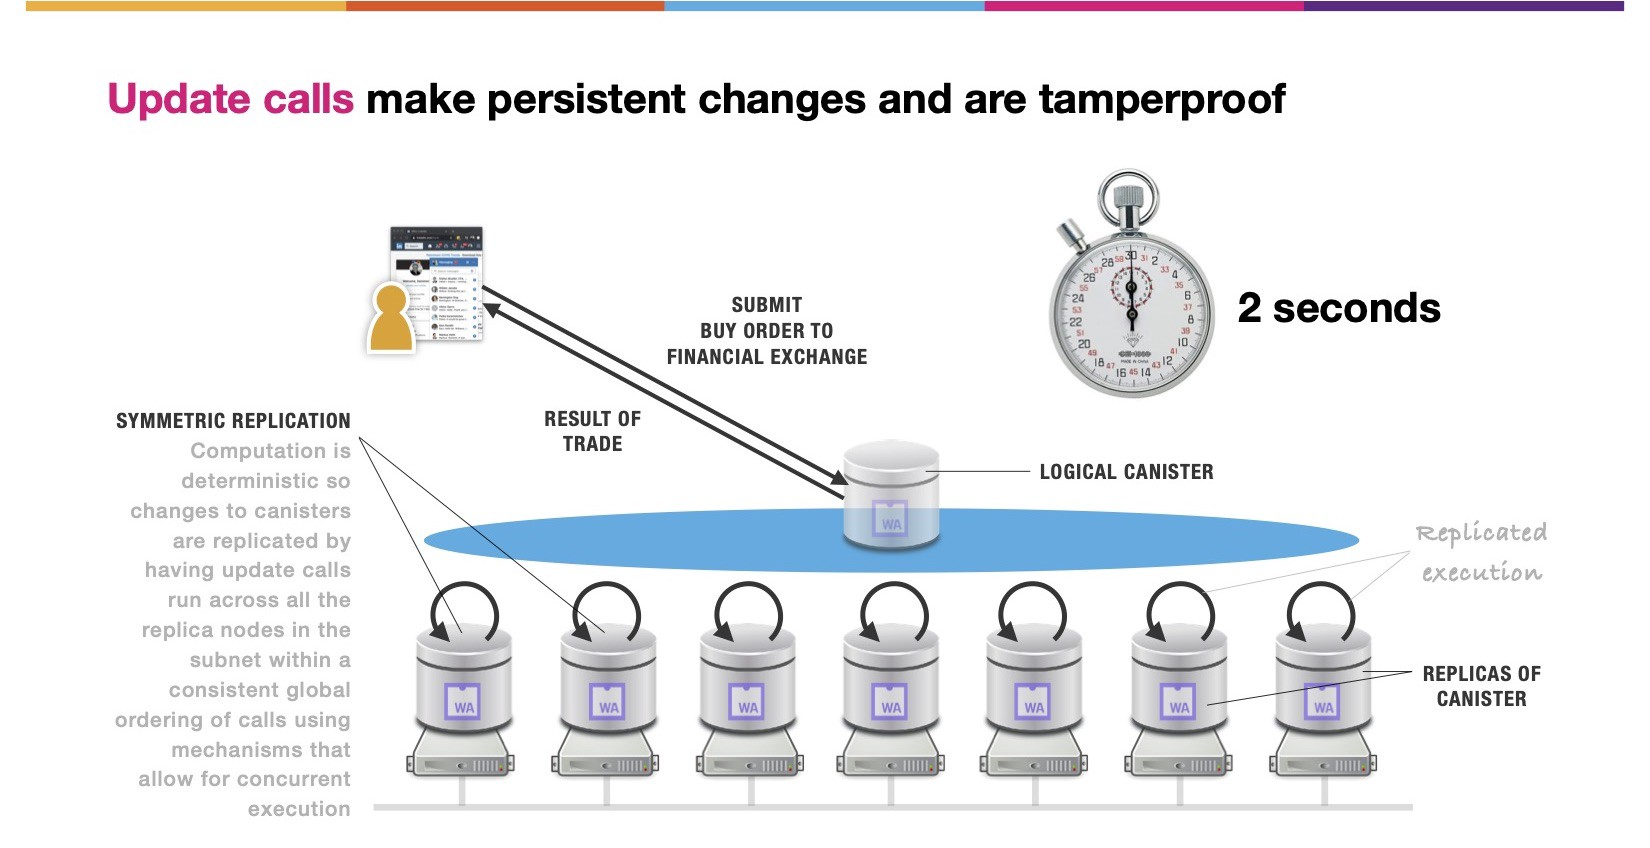
\includegraphics[width=0.8\textwidth]{update-calls.jpeg}
    \caption{Update call.}
    \label{fig:Update Call}
\end{figure}

The \textit{withDraw} function enables the user to withdraw money from their account. The amount parameter specifies the amount to be withdrawn. The function checks if the withdrawal amount is less than or equal to the \textit{currentValue}. If so, it subtracts the amount from the \textit{currentValue} and prints the updated balance. If the withdrawal amount exceeds the available balance, it prints a message indicating that the user does not have enough money.


The \textit{getBalance} function is a query function as shown in Figure \ref{fig:Query Call} that allows other actors or clients to retrieve the current balance asynchronously. It returns the \textit{currentValue} of the bank account.

\begin{figure}[H]
    \centering
    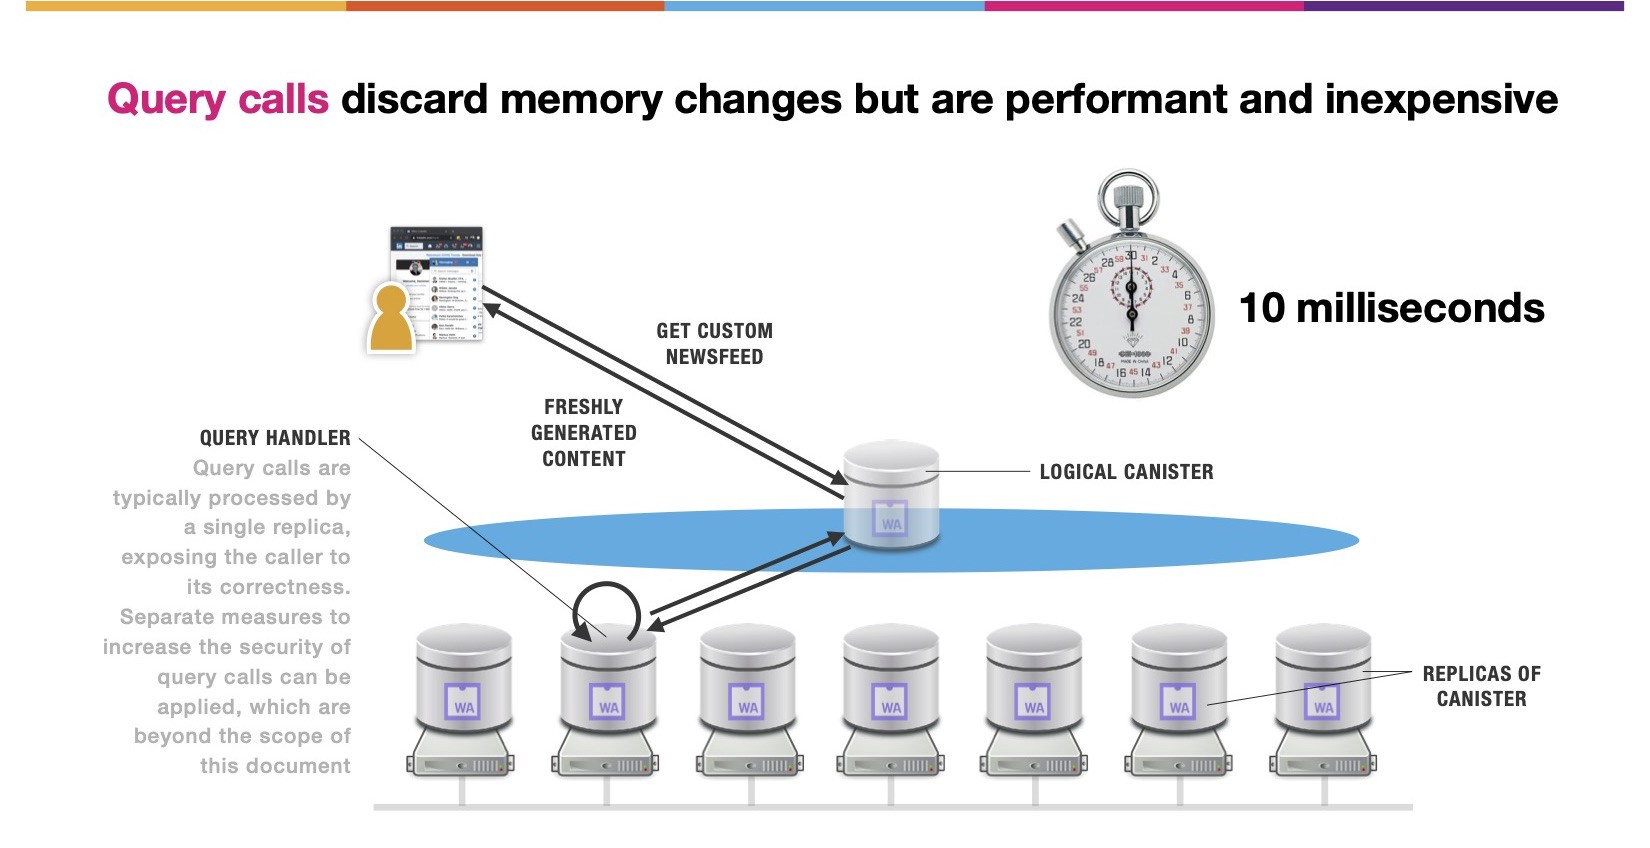
\includegraphics[width=0.8\textwidth]{query-calls.jpeg}
    \caption{Query Call.}
    \label{fig:Query Call}
\end{figure}

The compound function calculates compound interest on the bank account balance. It calculates the time difference between the current time and the \textit{startTime} and converts it to seconds. Then, it applies a compound interest formula to update the \textit{currentValue} by multiplying it with a factor of 1.01 raised to the power of the time difference in seconds. Finally, it updates the \textit{startTime} to the current time.

By incorporating this code into your implementation subsection, you can explain how the DBank actor manages bank accounts, allowing users to deposit, withdraw, check their balance, and earn compound interest on their funds over time.

\subsubsection{Frontend}

To handle the frontend part of the application, I utilized the following code in Figure \ref{fig:Frontend Implementation Code}:


\begin{figure}[h]
    \centering
    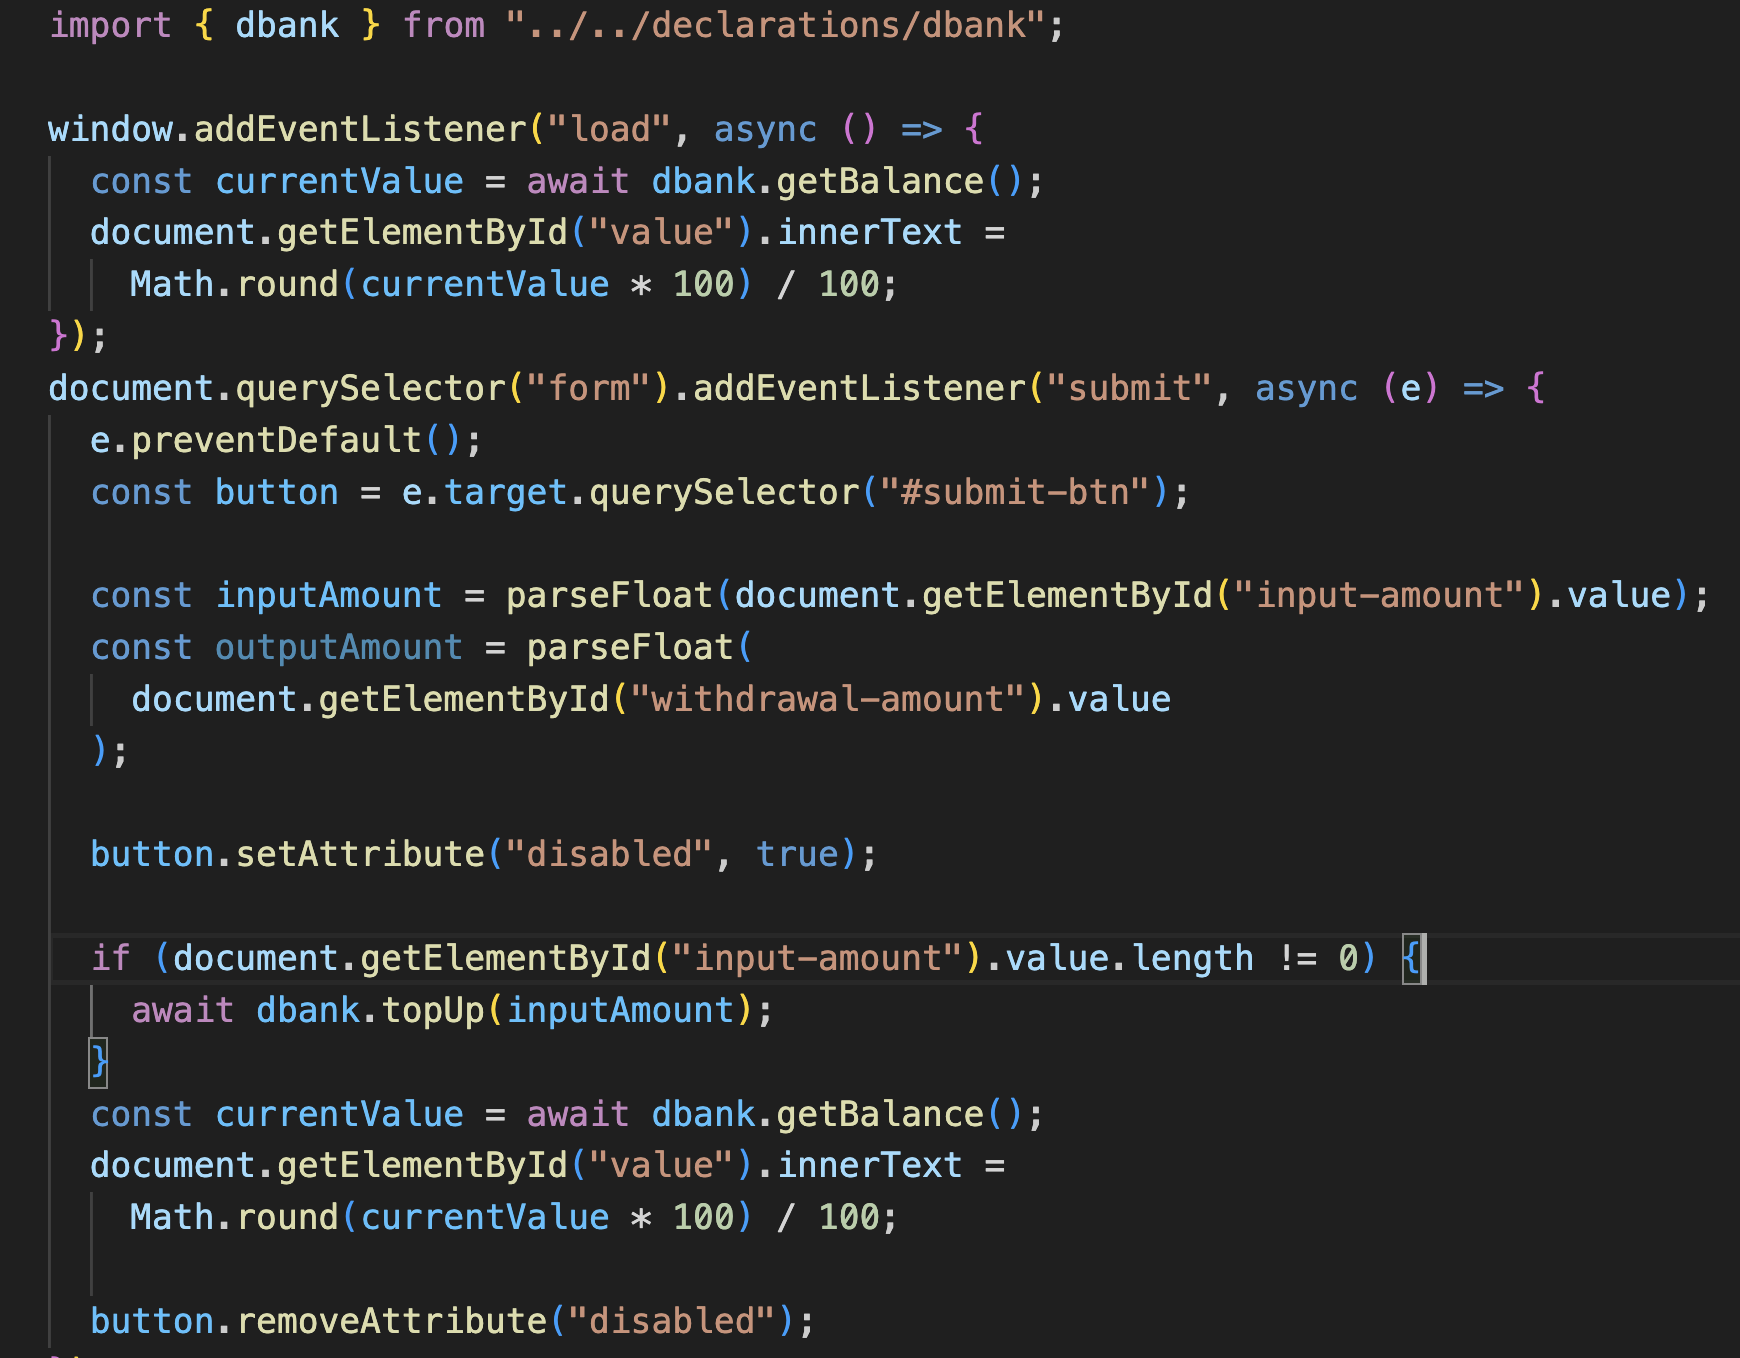
\includegraphics[height=1\textwidth, width=1\textwidth]{frontend.png}
    \caption{Frontend Implementation Code.}
    \label{fig:Frontend Implementation Code}
\end{figure}

This code snippet is responsible for interacting with the frontend elements of the application. It first listens for the "load" event on the window, ensuring that the page has fully loaded before executing the code inside the event listener. Inside the event listener, the current balance is fetched from the dbank canister using the getBalance function. The retrieved balance is then displayed on the webpage by updating the corresponding HTML element. Furthermore, the code sets up an event listener for the form submission. When the form is submitted, the function inside the event listener is triggered. It retrieves the values entered in the input fields for the amount to be deposited and the amount to be withdrawn. The submit button is temporarily disabled to prevent multiple submissions while the transaction is being processed. If an input amount is provided, the topUp function from the dbank canister is called to perform the deposit. After the transaction is completed, the current balance is fetched again, and the updated balance is displayed on the webpage. Finally, the submit button's disabled attribute is removed, allowing subsequent transactions to be made. By utilizing this code, the frontend of the application interacts with the backend canister functions, enabling users to perform actions such as depositing funds and retrieving the current balance.